\documentclass[aps,prl,reprint]{revtex4-1}
\usepackage{blindtext}

\usepackage{amsmath}
\usepackage{graphicx}
\usepackage{commath}
\usepackage{siunitx}
\usepackage{tabularx}
\usepackage{subcaption}

\usepackage{amssymb}

\usepackage{float}

\usepackage{graphicx}


\usepackage[b]{esvect}


\newcommand{\de}{\mathrm{d}}
\newcommand{\vcc}{V_\text{CC}}
\newcommand{\parallelsum}{\mathbin{\!/\mkern-5mu/\!}}


\graphicspath{ {images/} }
\begin{document}

\title{Unit 7: Comparitors, Converters and Computers}
\author{Xueqi Li}
% \email{xueqi.li@stonybrook.edu}
\thanks{Partner: Tianming Hai}
\noaffiliation
\date{May 4, 2018}



% \begin{abstract}
% In this lab we introduced operational amplifier and the negative feedback. Furthermore, a few importent applications of amplifier, such as follower, inverting and non-inverting amplifier, integrator, and differentiator were discussed and their output voltage formulas have been derived. Moreover, the limit of the opamp was explored and two methods to measure the slew rate have been given as examples.
% \end{abstract}

\maketitle

\section{Introduction}
    One can translate a analog signal into digital signal, or trnaslate digital signal to analog. In here, we introduce the rule we want to translate the signal.
    \subsection{Translation Rule}
    In here we want to have a ``bijective'' function between agalog signal and digital. The set of the analog signal is just a interval of real number, let say $[V_i,V_f]$, and the set of the digital is a binary number with some fix length, let say $\mathbb{B}^n$, where $n$ is the length of the binary number string. 

    We see that it is not possible to have a real bijective function, since $|[V_i, V_f]| \neq |\mathbb{B}^n|$ but we can do that with some resolution, depend on $n$. The number can be represent for a $n$ length binary number is $2^n$, which is the resolution we can have. Thus, we can think analog signal is a set of interval as following:
    \[
    \{[V_i, V_i + \frac{\Delta V}{2^n}),[V_i + \frac{\Delta V}{2^n}, V_i + 2\frac{\Delta V}{2^n})\cdots [V_f - \frac{\Delta V}{2^n},V_f]\}
    \]
    where $\Delta V = V_f - V_i$, Let define $a_k:=[V_i + k \frac{\Delta V}{2^n}, V_i + (k+1)\frac{\Delta V}{2^n})$, Thus we have:
    \begin{align*}
        \mathbb{A} &= \{[V_i + k \frac{\Delta V}{2^n}, V_i + (k+1)\frac{\Delta V}{2^n}): k \le 2^n - 1\}\\
                   &= \{a_k:k\in \mathbb{Z},0 \le k \le 2^n - 1\}
    \end{align*}
    Now we see it is possible to define a bijective between $\mathbb{A}$ to $\mathbb{B}^n$ since $|\mathbb{A}| = 2^n = |\mathbb{B}^n|$. Thus, we can defined our fucntion as following:
    \begin{align*}
        \Lambda(a_k) &= \text{Bin}\lfloor k\rfloor ;\\
        \Lambda^{-1}(b) &= a_{\text{Dec}(b)}
    \end{align*}
    where $\text{Bin}: \mathbb{R} \rightarrow \mathbb{B}^n$ maps a real number's interger part to its binary string and its ``inverse'' function is $\text{Dec}: \mathbb{B}^n \rightarrow \mathbb{Z}$ maps the binary string to the number it represent.

    We can defined $\varsigma$ to be the function gives the infimum of $a_k\in\mathbb{A}$ as following:
    \begin{align*}
        \varsigma(a_k) &= \inf(a_k) = V_i + k \frac{\Delta V}{2^n};\\
        \varsigma^{-1}(V)&= a_{\lfloor(V-V_i)\frac{2^n}{\Delta V} \rfloor}
    \end{align*}

    Than the translation between analog and digital signal is juat the composition of $\varsigma$ and $\Lambda$:
    \begin{align}
        \Xi (V) &= \varsigma^{-1} \circ \Lambda (V) = \text{Bin}\lfloor (V-V_i)\frac{2^n}{\Delta V} \rfloor;\label{eq:anaToDig}\\
        \Xi^{-1} (b)&= \Lambda^{-1} \circ \varsigma(V) = V_i + \text{Dec}(b) \frac{\Delta V}{2^n} \label{eq:digToAna}
    \end{align}

    \subsubsection{Zero Minimum Voltage}
        Let say if we have $V_i = 0$, $V_f = V_\text{ref}$. We see that $\Delta V = V_\text{ref}$. Thus the Equation~\ref{eq:anaToDig} and Equation~\ref{eq:digToAna} reduced to
        \begin{align}
            \Xi_0 (V) &= \text{Bin}\lfloor V\frac{2^n}{V_\text{ref}} \rfloor; \label{eq:anaToDig.zero}\\ 
            \Xi^{-1}_0 (b)&= \text{Dec}(b) \frac{V_\text{ref}}{2^n} \label{eq:digToAna.zero}
        \end{align}
\section{Data and Calculation}
    In the lab we are using ADC and DAC chip to translate digital and analog signal back and forth.

\section{Analysis}


\section{Conclusion}



\bibliography{cite}
\bibliographystyle{apsrev4-1}

    % \begin{figure}[h]
    %     \centering
    %     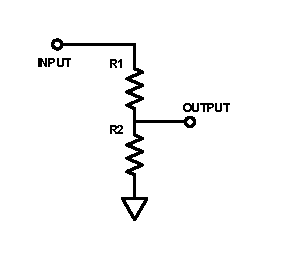
\includegraphics{images/plot2.pdf}
    %     \caption{A voltage divider}
    %     \label{fig:2}
    % \end{figure}

    % \begin{table}[h]
    % \begin{ruledtabular}
    % \begin{tabular}{cccc} 
    % Load[k$\Omega$] &  Output Voltage[V] & $R_\text{th}[\Omega]$ & Theoretical Voltage\\ \hline\hline
    % 50              & 0.680(1)           & 501(1)                & 0.682 \\ \hline
    % 500             & 3.75(1)            & 500(1)                & 3.75 \\ \hline
    % 5000            & 6.80(1)            & 514(1)                & 6.82 \\
    % \end{tabular}
    % \end{ruledtabular}
    % \caption{Load resistor and the output}
    % \label{table:8}
    % \end{table} 

% \begin{center}
%  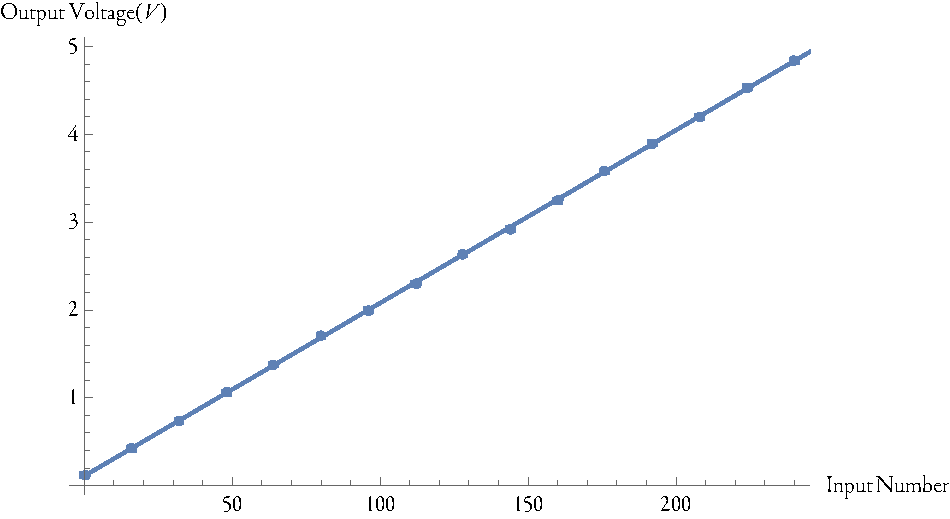
\includegraphics[height=1.8in]{plot.pdf}
% \end{center} 

%\begin{center}
% 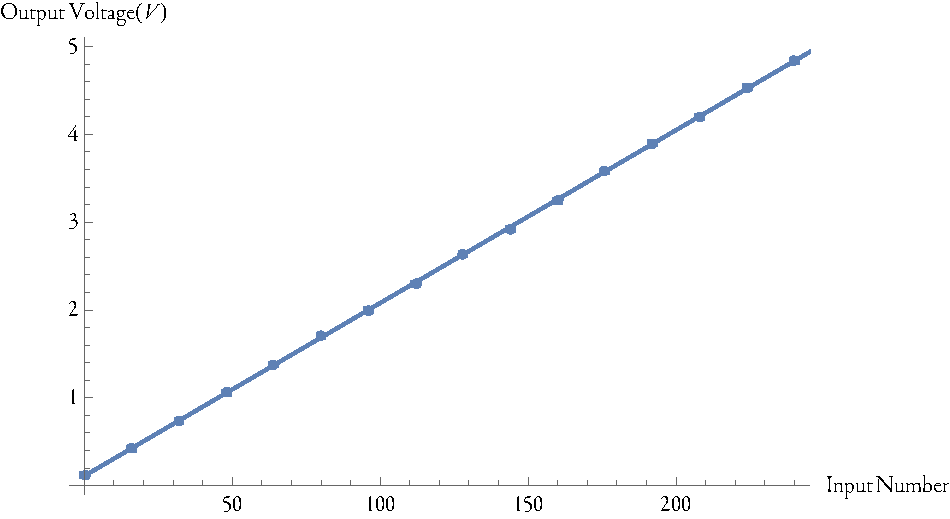
\includegraphics[height=1.3in]{plot.pdf}
%\end{center}

% \blindtext \cite{article-minimal}

% \bibliographystyle{apsrev4-1} % Tell bibtex which bibliography style to use
% \bibliography{xampl} % Tell bibtex which .bib file to use (this one is some example file in TexLive's file tree)

\end{document}